\subsection{FieldList}

FieldList indeholder et array af felter. Alle felterne, som forekommer på spilbrættet, bliver beskrevet i denne klasse.
\begin{figure}[H]
    \centering
    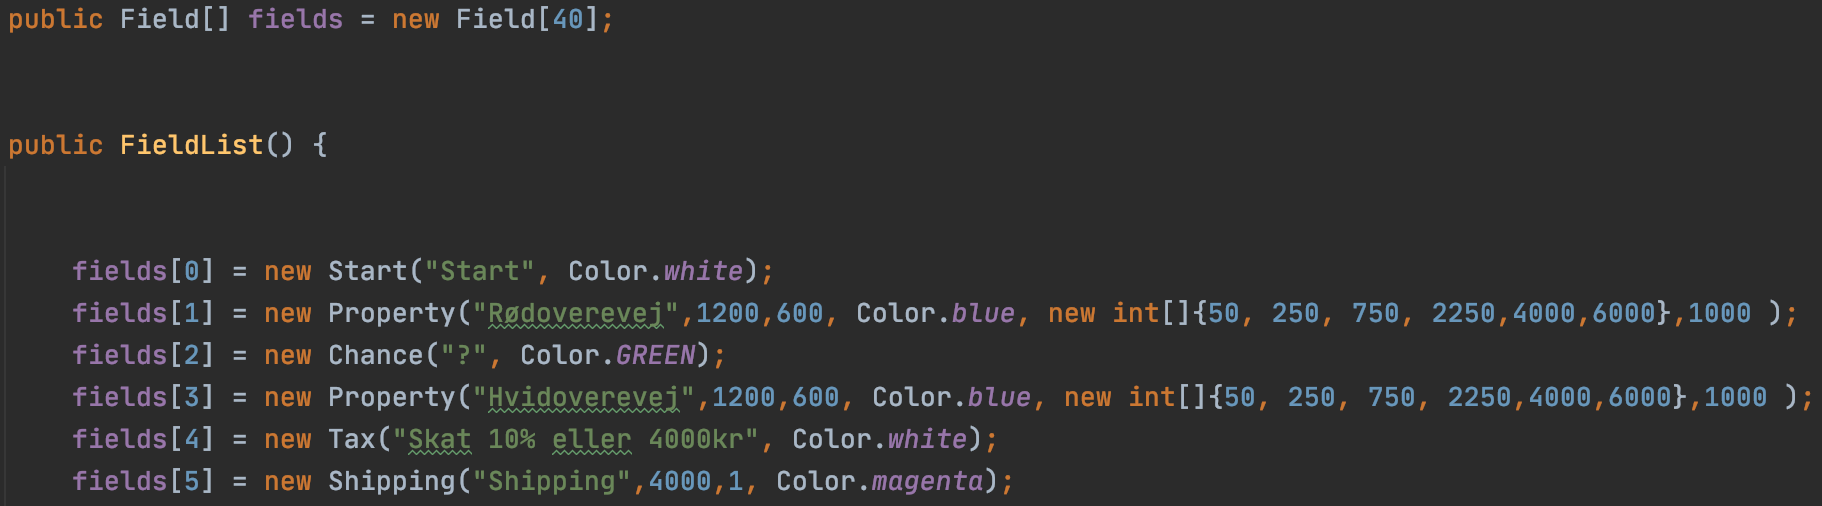
\includegraphics[width=\textwidth]{sources/7_implementering/FieldList FieldList.png}
    \caption{Array af felter i FieldList}
    \label{fig:FieldListArray}
\end{figure}
Vi har en række forskellige felter, som stemmer overens med dem, som forekommer på spilbrættet. De har hver især en række forskellige variable, som bruges i beskrivelsen af dem. F.eks. en farve til feltet, eller en pris på en grund.
Klassen gør brug af informationen fra vores field klasser til at oprette dette array.


Vi har en getField metode, som er en getter til felterne. Den bruges bl.a. til at se, hvilket felt en spiller er landet på i GameControlleren, så et bestemt udfald kan forekomme.
Sidst er en getSize metode, som ligeledes er en getter blot for størrelsen af vores array.
\begin{figure}[H]
    \centering
    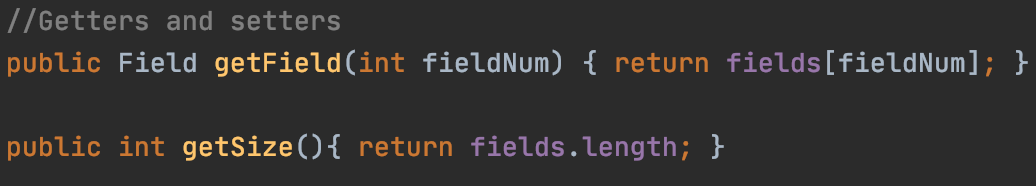
\includegraphics[width=\textwidth]{sources/7_implementering/FieldList Getters}
    \caption{FieldList getters}
    \label{fig:FieldList Getters}
\end{figure}